In this section, you will describe all of the various artifacts that you will generate and maintain during the project lifecycle. Describe the purpose of each item below, how the content will be generated, where it will be stored, how often it will be updated, etc. 

\subsection{Project Charter}
Details for the project charter are contained within this document.

\subsection{Product Backlog}
\begin{table}[htbp]
    \centering
    \begin{tabularx}{\textwidth}{l}
        Task\\
        \hline
        Investigate Neural Network Python Packages\\
        Create Bare-bones Android Application\\
        Implement server-side code on AWS\\
    \end{tabularx}
\end{table}

\subsection{Sprint Work}
In this section we detail the work done during each sprint.
\subsubsection{Sprint 1}

\paragraph{Sprint Goal}
\begin{itemize}
    \item  Develop an understanding of basic human speech, neural networks, Fourier transform, and Formant frequencies.
    \item  Gather all data and supplies required for Android application development.
\end{itemize}

\paragraph{Sprint Backlog}
\begin{tabular}[htbp]
    \centering
    \begin{tabularx}{\textwidth}{l|l|l|l|l|l|l}
        User Story & Tasks &    Mon & Tue & Wed & Thur & Fri\\
        \hline
        & Research on basic human speech features & 3 & 3 & 3 & 3 & 0\\
        & Research on neural networks & 3 & 3 & 3 & 3 & 0\\
        & Research on Fourier transforms and Format frequencies & 2 & 2 & 0 & 0 & 0\\
        & Record samples of common US English (enUS) words & 1 & 1 & 0 & 0 & 0\\
        1 & Learn Javascript and HTML & 1 & 1 & 1 & 1 & 1\\
        1 & Create a webpage using JavaScript and HTML & 1 & 1 & 1 & 1 & 1\\
        1 & Design Web Interface & 1 & 1 & 1 & 1 & 1\\
        1 & Test the program & 1 & 1 & 1 & 1 & 1\\
        2 & Download proper Android development software & 1 & 0 & 0 & 0 & 0\\
        2 & Implement recording option for the user & 1 & 1 & 1 & 1 & 1\\
        2 & Store recorded word & 2 & 0 & 0 & 0 & 0\\
        2 & Display the word on the screen as a plot & 2 & 2 & 0 & 0 & 0\\
        & Research on various python libraries & 2 & 0 & 0 & 0 & 0\\
        & Implement Fourier transform, Formant frequency, and spectrogram in Python. Use a speech signal (word) as a sample & 4 & 4 & 4 & 4 & 4\\
    \end{tabularx}
\end{tabular}
\begin{table}[htbp]
    \centering
    \begin{tabularx}{\textwidth}{l|l}
        User Story No. & Description\\
        \hline
        1 & Build an API on mobile platform\\
        1 & Build a prototype in Android Studio\\
    \end{tabularx}
\end{table}

\paragraph{Task Breakdown}
\begin{table}[htbp]
    \centering
    \begin{tabularx}{\textwidth}{l|l}
        Backlog Item & Est. Time\\
        \hline
        Research on basic human speech features & 12\\
        Research on neural networks & 12\\
        Research on Fourier transform and Formant frequencies & 4\\
        Record samples of common US English (enUS) words & 2\\
        Build an API on a mobile platform to send the input to the server, properly display output & 14\\
        Build a prototype in Android studio & 12\\
        Research on various Python libraries & 2\\
        Implement Fourier transform, Formant frequency, and spectrogram in Python. & 10\\
        Use a speech signal (word) as a sample & 10\\
        Gather information on cloud development & 4\\
    \end{tabularx}
\end{table}

\paragraph{Sprint Retrospective}
In Sprint 1, we completed our research on basic human speech features, neural networks, and Fourier transform and Formant frequencies. We also researched what we would need our server to do and what environment to work in. We recorded samples of 100 common US English words for the database. We are still working on implementing Fourier transform, Formant frequency, and spectogram. We are also still int eh process of building a prototype of our app.


\subsubsection{Sprint 2}

\paragraph{Sprint Goal}
\begin{itemize}
    \item  Ensure compatibility on all platforms such as Android, Apple, and Windows using Xamarin or other development tools.
    \item  Gather all data and supplies required for Android application development.
\end{itemize}

\paragraph{Sprint Backlog}
\begin{table}[htbp]
    \centering
    \begin{tabularx}{\textwidth}{l|l}
        Backlog Item & Est. Time\\
        \hline
        Build a prototype in Xamarin or Android Studio & 12\\
        Implement Fourier transform, Formant frequency, and spectogram & 12\\
        Create SRS documentation & 4
    \end{tabularx}
\end{table}

\paragraph{Task Breakdown}
\begin{tabular}[htbp]
    \centering
    \begin{tabularx}{\textwidth}{l|l|l|l|l|l|l}
        Tasks &    Mon & Tue & Wed & Thur & Fri\\
        \hline
        Implement recording option for user & 2 & 1 & 1 & 1 & 0\\
        Store the recorded words & 1 & 1 & 0 & 0 & 0\\
        Display the word on the screen as a plot & 2 & 1 & 1 & 1 & 0\\
        Research on various Python libraries & 2 & 3 & 2 & 3 & 2\\
        Create SRS documentation & 2 & 2 & 0 & 0 & 0\\
    \end{tabularx}
\end{tabular}

\paragraph{Sprint Retrospective}
In Sprint 2, we completed the SRS documentation and implemented the Fourier transform, Formant frequenct, and spectogram in python. We are still trying to decide if we want to implement the app only in Android Studio or if it should be written in Xamarin so that it can be used by Apple devices as well.


\subsubsection{Sprint 3}

\paragraph{Sprint Goal}
\begin{itemize}
    \item  Design prototype.
    \item  Complete ADS (architectural design specification.
\end{itemize}

\paragraph{Sprint Backlog}
\begin{table}[htbp]
    \centering
    \begin{tabularx}{\textwidth}{l|l}
        Backlog Item & Est. Time\\
        \hline
        Build a prototype in Xamarin or Android Studio & 20\\
        Create ADS documentation & 4\\
    \end{tabularx}
\end{table}

\paragraph{Task Breakdown}
\begin{tabular}[htbp]
    \centering
    \begin{tabularx}{\textwidth}{l|l|l|l|l|l|l}
        Tasks &    Mon & Tue & Wed & Thur & Fri\\
        \hline
        Implement recording option for user & 2 & 2 & 2 & 2 & 1\\
        Store the recorded words & 1 & 1 & 0 & 0 & 0\\
        Display the word on the screen as a plot & 2 & 2 & 2 & 2 & 1\\
        Create ADS documentation & 2 & 2 & 0 & 0 & 0\\
    \end{tabularx}
\end{tabular}

\paragraph{Sprint Retrospective}
In Sprint 3, we finished designing the prototype and decided to use Android Studio only. This means that our app will only run on Android devices. We also finished our ADS documentation. We are still in the process of building the prototype in Android Studio.


\subsubsection{Sprint 4}

\paragraph{Sprint Goal}
\begin{itemize}
    \item  Expand UML diagram for server-side to include additional details.
    \item  Start implementing sever-side architecture.
    \item  Continue to build the prototype in Android Studio.
\end{itemize}

\paragraph{Sprint Backlog}
\begin{table}[htbp]
    \centering
    \begin{tabularx}{\textwidth}{l|l}
        Backlog Item & Est. Time\\
        \hline
        Get login information for server from Digital Ocean & 5\\
        Build a prototype in Android Studio & 10\\
        Finish UML diagram for server-side architecture & 7\\
    \end{tabularx}
\end{table}

\paragraph{Task Breakdown}
\begin{tabular}[htbp]
    \centering
    \begin{tabularx}{\textwidth}{l|l|l|l|l|l|l}
        Tasks &    Mon & Tue & Wed & Thur & Fri\\
        \hline
        Finish UML diagram for server-side architecture & 2 & 0 & 0 & 0 & 0\\
        Test SSH and SFTP access & 0 & 1 & 0 & 0 & 0\\
        Set up a dummy web service & 1 & 0 & 0 & 0 & 0\\
        Begin implementing server-side architecture & 0 & 0 & 2 & 2 & 2\\
        Get app to run on phone and connect to server-side dummy web service & 2 & 2 & 2 & 2 & 2\\
    \end{tabularx}
\end{tabular}

\paragraph{Sprint Retrospective}
In Sprint 4, we expanded the UML diagram to include all additional details for the server-side architecture. We were also able to test the SSH and SFTP access to make sure they connect to the dummy web service. An empty app was made that only connected to the dummy web service and was able to confirm that it connected. We are still working on implementing the server-side architecture.


\subsubsection{Sprint 5}

\paragraph{Sprint Goal}
\begin{itemize}
    \item  Finish STP documentation.
    \item  Start implementing sever-side architecture.
    \item  Continue to build the prototype in Android Studio and make changes.
\end{itemize}

\paragraph{Sprint Backlog}
\begin{table}[htbp]
    \centering
    \begin{tabularx}{\textwidth}{l|l}
        Backlog Item & Est. Time\\
        \hline
        Start implementing server-side architecture & 6\\
        Continue to build a prototype in Android Studio & 10\\
        Finish STP documentation & 2\\
    \end{tabularx}
\end{table}

\paragraph{Task Breakdown}
\begin{tabular}[htbp]
    \centering
    \begin{tabularx}{\textwidth}{l|l|l|l|l|l|l}
        Tasks &    Mon & Tue & Wed & Thur & Fri\\
        \hline
        Start implementing server-side architecture & 2 & 0 & 2 & 0 & 2\\
        Continue to build prototype in Android Studio & 2 & 2 & 2 & 2 & 2\\
        Finish STP documentation & 0 & 1 & 0 & 1 & 0\\
    \end{tabularx}
\end{tabular}

\paragraph{Sprint Retrospective}
In Sprint 5, we completed the STP documentation and the server-side architecture. We are still working on building the app in Android Studio.


\subsubsection{Sprint 6}

\paragraph{Sprint Goal}
\begin{itemize}
    \item  Finish implementing server-side architecture.
    \item  Continue to build app in Android Studio.
\end{itemize}

\paragraph{Sprint Backlog}
\begin{table}[htbp]
    \centering
    \begin{tabularx}{\textwidth}{l|l}
        Backlog Item & Est. Time\\
        \hline
        Finish implementing server-side architecture & 4\\
        Continue to build app in Android Studio & 12\\
        DDS documentation & 2\\
    \end{tabularx}
\end{table}

\paragraph{Task Breakdown}
\begin{tabular}[htbp]
    \centering
    \begin{tabularx}{\textwidth}{l|l|l|l|l|l|l}
        Tasks &    Mon & Tue & Wed & Thur & Fri\\
        \hline
        Fix bugs in server-side architecture & 1 & 1 & 1 & 1 & 0\\
        Establish JSON connection to AWS back-end & 2 & 0 & 2 & 0 & 0\\
        Pass Audio file along with string text of word spoken & 0 & 2 & 0 & 0 & 2\\
        Return an output in the format of JSON back to the front-end & 0 & 0 & 0 & 2 & 2\\
        DDS documentation & 1 & 1 & 0 & 0 & 0\\
    \end{tabularx}
\end{tabular}

\paragraph{Sprint Retrospective}
In Sprint 6, we completed the DDS documentation and the server side architecture. We have the app in Android Studio and are still in the process of testing it.


\subsubsection{Sprint 7}

\paragraph{Sprint Goal}
\begin{itemize}
    \item  Finish testing the app.
    \item  Test the connection between the server and the application.
\end{itemize}

\paragraph{Sprint Backlog}
\begin{table}[htbp]
    \centering
    \begin{tabularx}{\textwidth}{l|l}
        Backlog Item & Est. Time\\
        \hline
        Update DDS & 2\\
        Application testing & 8\\
        Test connection between server and client & 6\\
    \end{tabularx}
\end{table}

\paragraph{Task Breakdown}
\begin{tabular}[htbp]
    \centering
    \begin{tabularx}{\textwidth}{l|l|l|l|l|l|l}
        Tasks &    Mon & Tue & Wed & Thur & Fri\\
        \hline
        Update DDS & 0 & 1 & 0 & 1 & 0\\
        Application testing & 2 & 0 & 5 & 1 & 0\\
        Test connection between server and client & 0 & 2 & 0 & 2 & 2\\
    \end{tabularx}
\end{tabular}

\paragraph{Sprint Retrospective}
In Sprint 7, we updated the DDS and continue testing the app. There are some minor bugs to work out but we are working on fixing them. The connection between the server and the client is working.


%%%\subsection{Sprint Burndown Charts}
%%%Lorem ipsum dolor sit amet, quidam omnesque ea vis. Eum an aliquip legendos recusabo. Mea ex purto natum, ne movet fuisset sit. Labore audiam eos ad, facer ornatus posidonium ne ius, et eos duis delenit nusquam.

%%%\begin{figure}[h!]
    %%%\centering
    %%%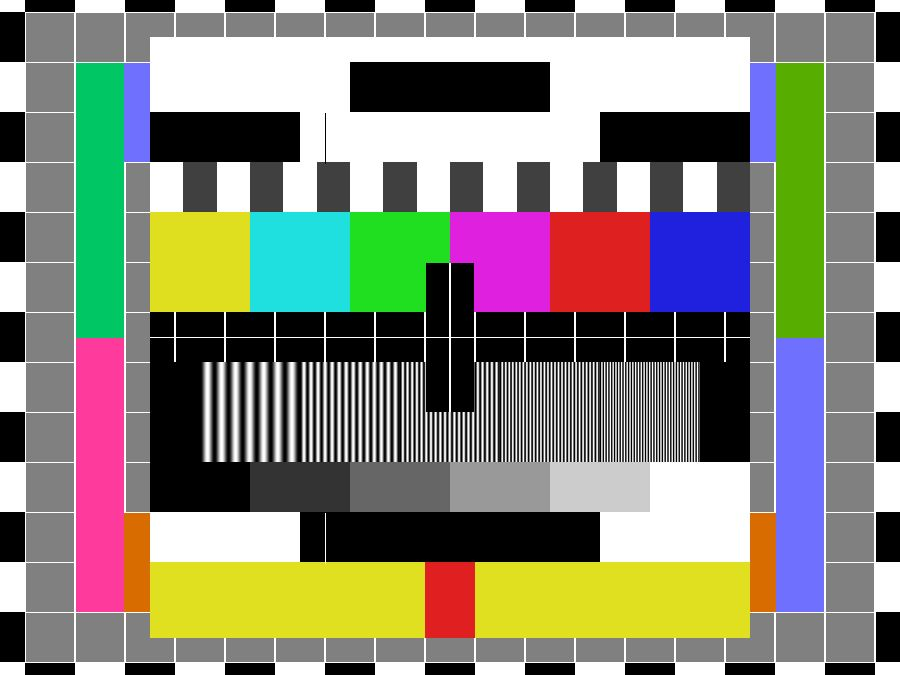
\includegraphics[width=0.5\textwidth]{figures/test_image}
    %%%\caption{Example sprint burndown chart}
%%%\end{figure}

%%%\subsection{Individual Status Reports}
%%%Lorem ipsum dolor sit amet, quidam omnesque ea vis. Eum an aliquip legendos recusabo. Mea ex purto natum, ne movet fuisset sit. Labore audiam eos ad, facer ornatus posidonium ne ius, et eos duis delenit nusquam.

\subsection{Engineering Notebooks}
Josue Caraballo:

Syed Ali:

Norween Jilaney:

Xiwen Du:

Kristen Rutherford:


\subsection{Closeout Materials}

%%%\subsubsection{System Prototype}
%%%Lorem ipsum dolor sit amet, quidam omnesque ea vis. Eum an aliquip legendos recusabo. Mea ex purto natum, ne movet fuisset sit. Labore audiam eos ad, facer ornatus posidonium ne ius, et eos duis delenit nusquam.

\subsubsection{Project Poster}
\begin{figure}[h!]
	\centering
   	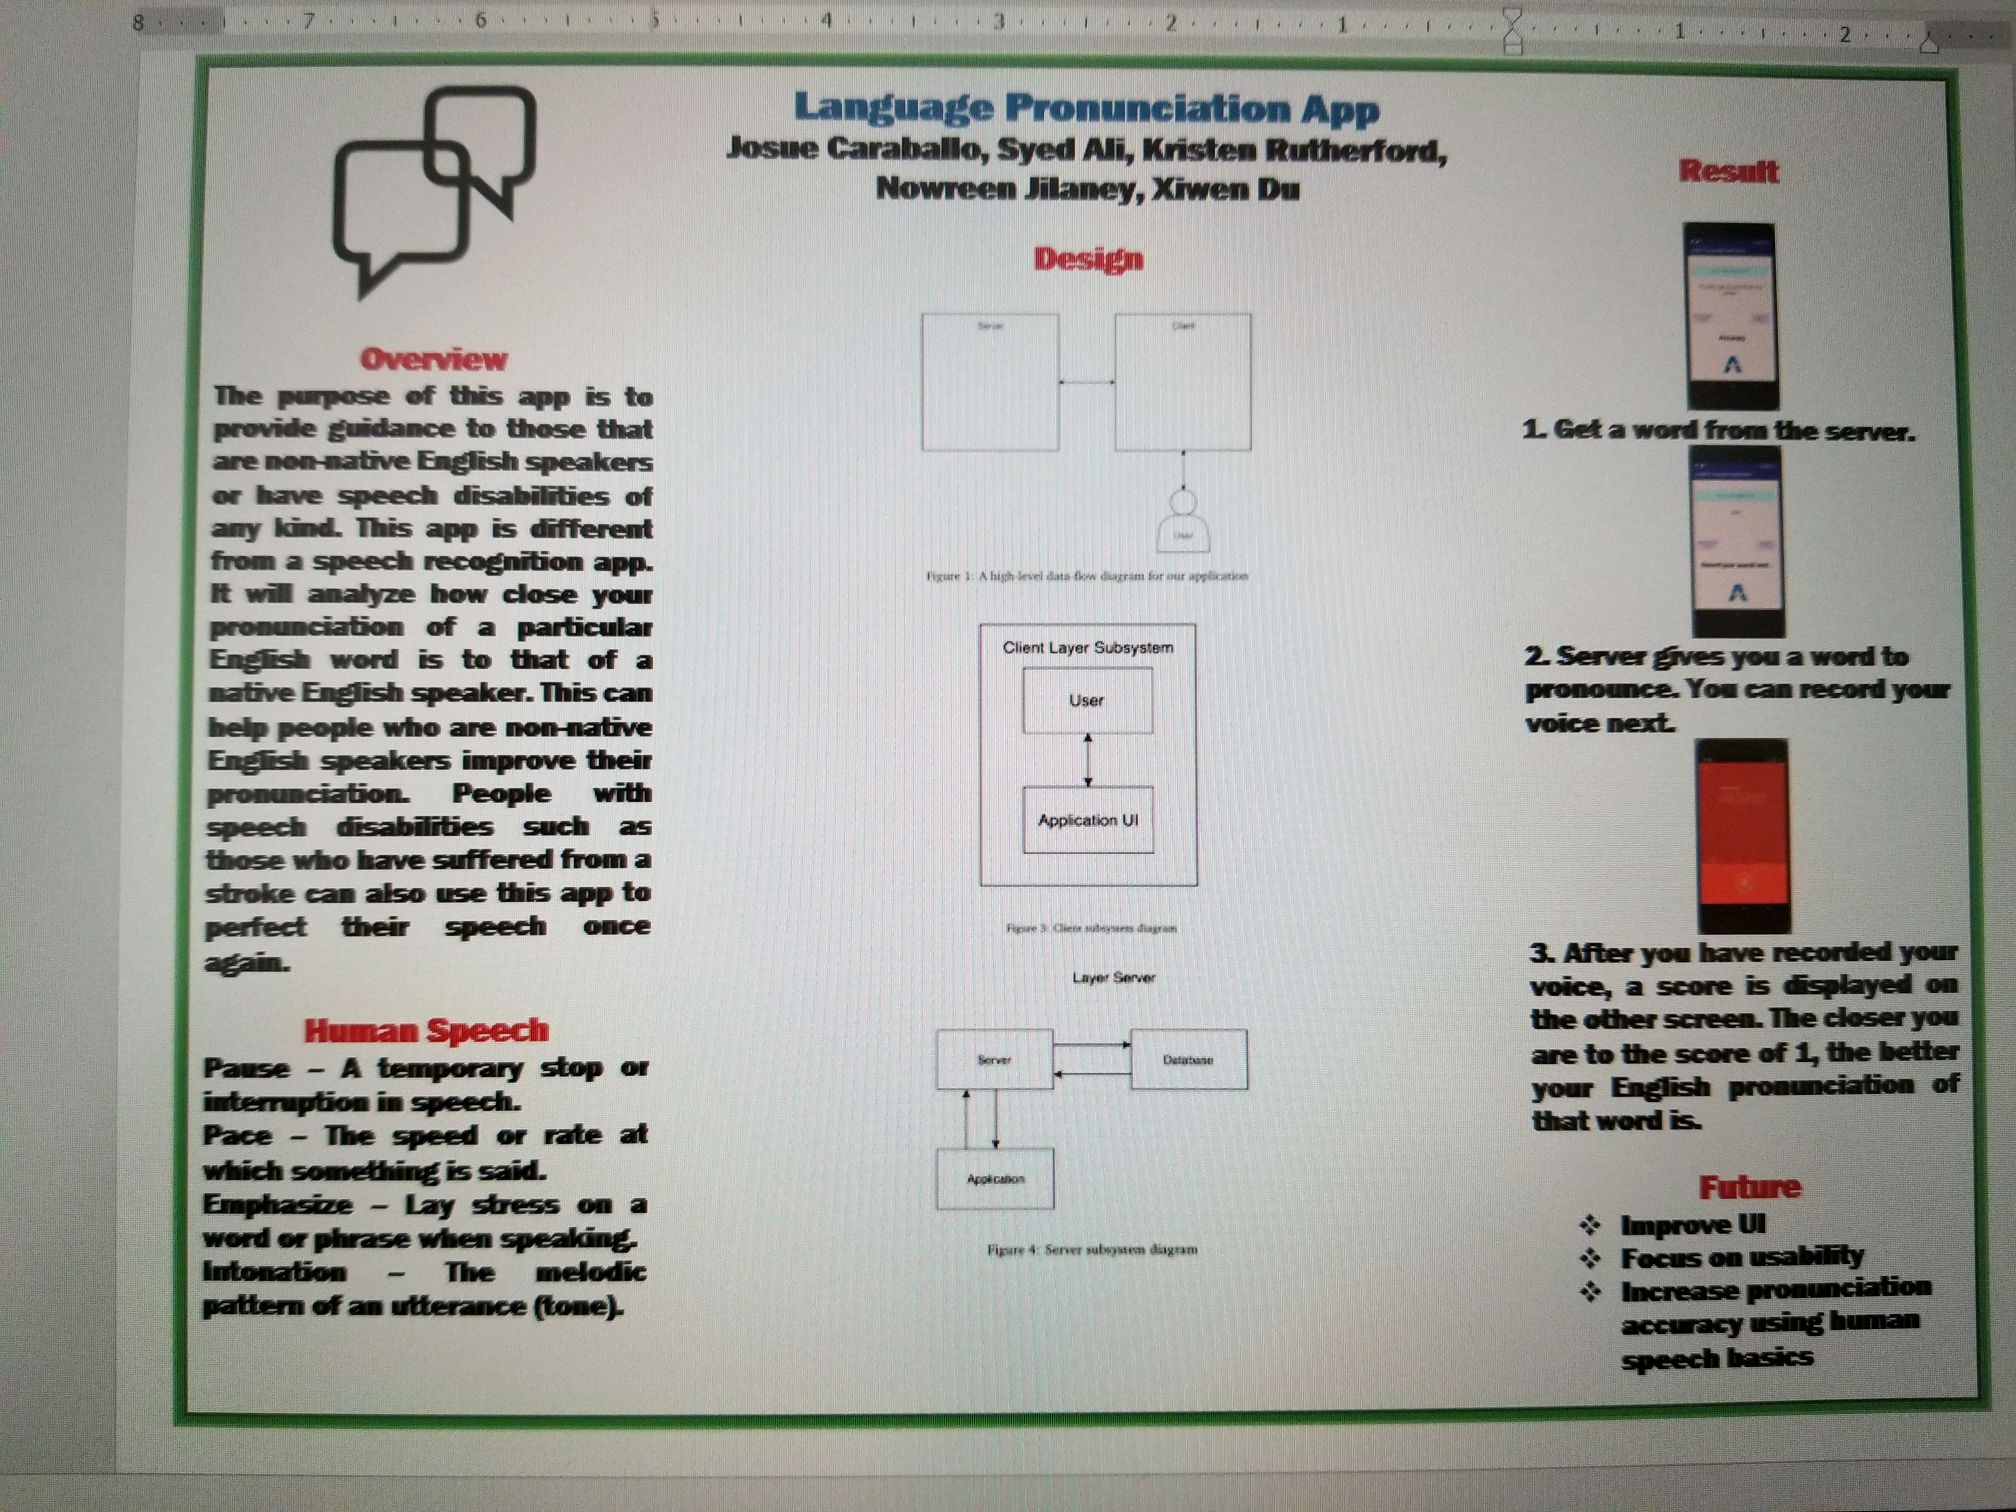
\includegraphics[width=1\textwidth]{figures/poster.jpeg}
\end{figure}

\subsubsection{Web Page}
Our website is located \href{https://sd2.000webhostapp.com/}{here}.

\subsubsection{Demo Video}
The demo video for our app is located on our \href{https://sd2.000webhostapp.com/}{website} under the Preview tab.

\subsubsection{Source Code}
Lorem ipsum dolor sit amet, quidam omnesque ea vis. Eum an aliquip legendos recusabo. Mea ex purto natum, ne movet fuisset sit. Labore audiam eos ad, facer ornatus posidonium ne ius, et eos duis delenit nusquam.

\subsubsection{Source Code Documentation}
Lorem ipsum dolor sit amet, quidam omnesque ea vis. Eum an aliquip legendos recusabo. Mea ex purto natum, ne movet fuisset sit. Labore audiam eos ad, facer ornatus posidonium ne ius, et eos duis delenit nusquam.

%%%\subsubsection{Hardware Schematics}
%%%Lorem ipsum dolor sit amet, quidam omnesque ea vis. Eum an aliquip legendos recusabo. Mea ex purto natum, ne movet fuisset sit. Labore audiam eos ad, facer ornatus posidonium ne ius, et eos duis delenit nusquam.

%%%\subsubsection{CAD files}
%%%Lorem ipsum dolor sit amet, quidam omnesque ea vis. Eum an aliquip legendos recusabo. Mea ex purto natum, ne movet fuisset sit. Labore audiam eos ad, facer ornatus posidonium ne ius, et eos duis delenit nusquam.

\subsubsection{Installation Scripts}
To install the app go to the Google Plus store to download it onto your Andriod phone.

\subsubsection{User Manual}
Lorem ipsum dolor sit amet, quidam omnesque ea vis. Eum an aliquip legendos recusabo. Mea ex purto natum, ne movet fuisset sit. Labore audiam eos ad, facer ornatus posidonium ne ius, et eos duis delenit nusquam.
